
\subsection{Solver loop}

Once \texttt{Reaction}s and \texttt{Reactant}s are defined,
they must be integrated properly.
We use variants of the Gillespie algorithm to provide a framework
where reactions are performed according to their current reaction rate.
Roughly speaking, the main hypothesis of this framework is that
reaction timings are distributed according to exponential distributions.
This allows for many mathematical simplifications and harmonious integration
of an arbitrary number of reactions.
The central point of the algorithm is that the probability that a reaction
will be the next reaction in the system is proportional to its rate
(mathematically speaking, the reaction is obtained by multinomial drawing according to rates).

\begin{figure}[!h]
  \centering
  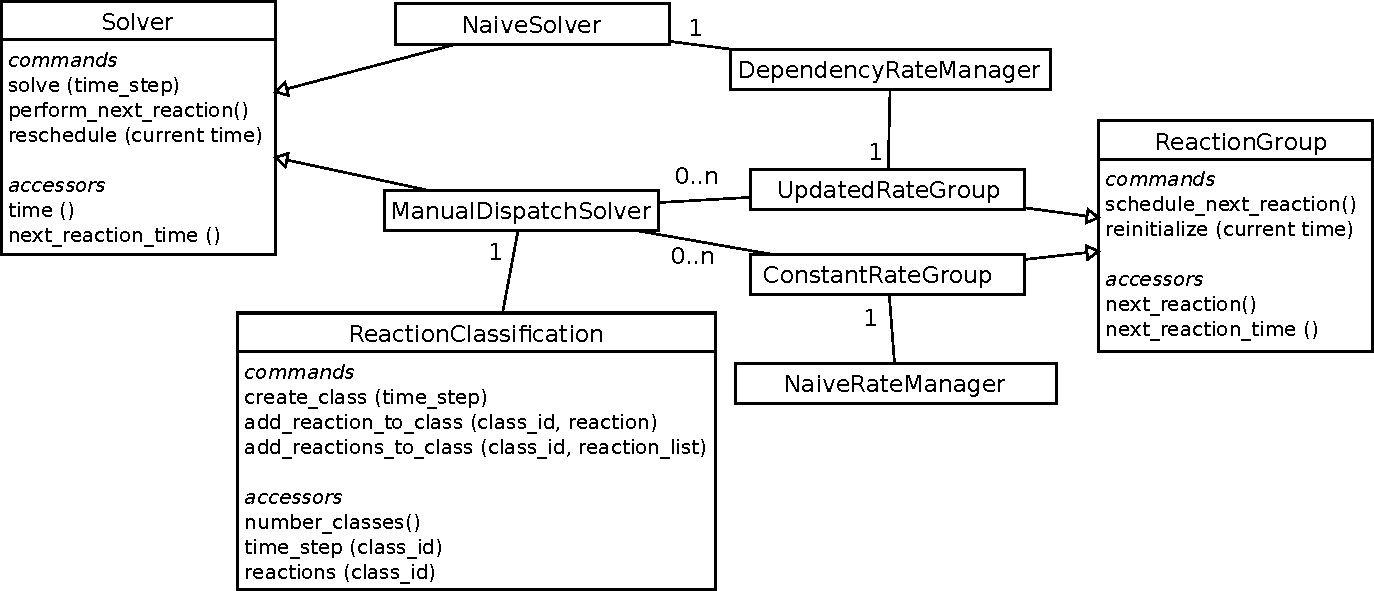
\includegraphics[width=\linewidth]{solver}
  \caption{Solver loop.
  The loop is driven by the \texttt{Solver} class that defines
  how and when rates should be updated.
  The update task is performed by a \texttt{RateManager}.
  Once rates are known, multinomial drawing is delegated to a \texttt{RateContainer}.
  A central \texttt{RandomHandler} is used so that the solver only uses one seed,
  enabling simulation reproducibility.}
\label{fig:solver}
\end{figure}

The solving loop is depicted in~\reffigt{fig:solver}.
The Gillespie algorithm has many variants.
We decided to implement it using three \emph{abstract} classes.
By using inheritance, variants can be combined for each step of the algorithm
(how to update reactions, how to select a reaction).
The three central classes are:
\begin{itemize}
  \item \texttt{Solver}:
  Children of this class decide how and when rates should be updated,
  \textit{e.g.} update rates after every reaction, only after a given time step, etc.
  Note that they do not perform any of these computations,
  they just organize how the algorithm should work.
  \item \texttt{RateManager}:
  Children of this class are responsible for updating reaction rates
  when prompted to by a \texttt{Solver} class.
  Recomputing all rates is generally inefficient,
  so various implementations of this task can be used to improve the global loop speed.
  \item \texttt{RateContainer}: Children of this class are responsible for storing reaction rates
  in a specific structure \emph{adapted} to multinomial drawing.
  Again many implementations exist, their efficiency depends on the system that is integrated.
\end{itemize}
The implementations of these three classes will be described later in the document.
